% Ten plik jest zaprojektowany do użycia z LuaLaTeX.

\documentclass[a4paper,12pt]{article}
\usepackage{fontspec} % Obsługa czcionek w LuaLaTeX
\usepackage[polish]{babel}
\usepackage{geometry} % Ustawienia marginesów
\geometry{margin=1in}
\usepackage{hyperref} % Obsługa hiperłączy
\usepackage{titlesec} % Formatowanie sekcji
\usepackage[skip=10pt plus1pt]{parskip}
\usepackage[table]{xcolor}
\usepackage{float}

\usepackage{graphicx}
\graphicspath{ {./images/} }

% Ustawienia hiperłączy
\hypersetup{
    colorlinks=true,
    linkcolor=black,
    urlcolor=blue,
    pdftitle={Podział pracy},
    pdfauthor={Diego Ostoja Kowalski}
}

% Tytuł dokumentu
\title{
    \line(1,0){250}\\
    System Zarządzania Promocjami\\
    Podział pracy\\
    \line(1,0){250}}
\author{Antoni Blicharz\\
        Szymon Dybał\\
        Jakub Koszorz\\
        Mikołaj Mroczek\\
        Diego Ostoja-Kowalski\\}
\date{\today}

\begin{document}

\begin{titlepage}
    \maketitle
\end{titlepage}

\newpage

\section{Wykres Gantta}

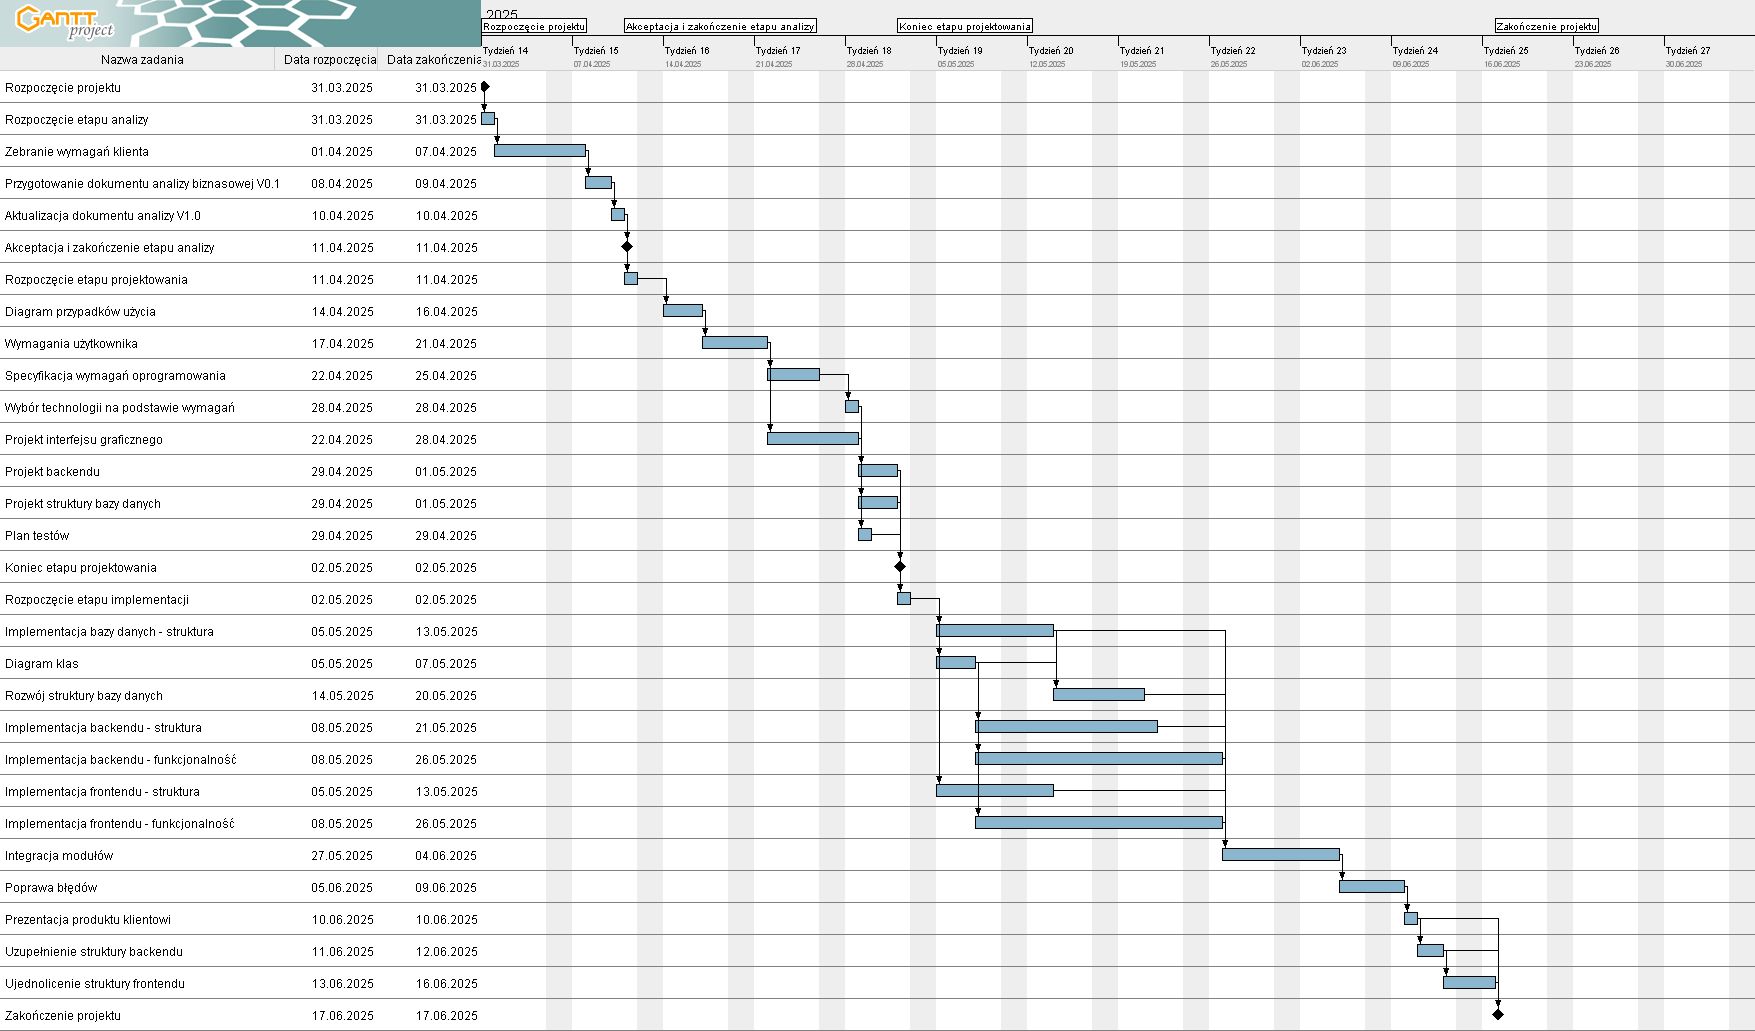
\includegraphics[width=\textwidth]{images/Gantt.png}

\section{Logi commitów}

Ze względu na problemy techniczne nie są dostępne wyciągi logów z repozytorium, ale są one dostępne w formie tekstowej w pliku \texttt{commit\textunderscore{}log.txt}.

\section{Podział pracy}

\begin{itemize}
    \item \textbf{Antoni Blicharz} -- testowanie oprogramowania, opis testów, przygotowanie prezentacji demo.
    \item \textbf{Szymon Dybał} -- postawienie bazy danych MySQL w AWS, utrzymywanie bazy danych i populowanie jej danymi testowymi, pomoc w komentowaniu kodu, instrukcja obsługi, implementacja generowania raportów PDF.
    \item \textbf{Jakub Koszorz} -- lider projektu, architektura frontendowa, postawienie bazy danych MySQL w AWS, panele analityka biznesowego.
    \item \textbf{Mikołaj Mroczek} -- wczesna eksploracja JavaFX, utworzenie szkieletu aplikacji (zarządzanie scenami i prototyp logiki aplikacji), wprowadzenie wzorca MVCS, łączność z bazą danych od strony języka Java, panele pracownika punktu sprzedaży.
    \item \textbf{Diego Ostoja-Kowalski} -- wizja projektu, utworzenie dokumentacji projektu, panele koordynatora promocji i koordynatora logistyki, części warstw Model i Service odpowiedzialne za tworzenie list i tabel obiektów.
\end{itemize}

\newpage

Specjalne podziękowania również idą w stronę \textbf{Kingi Żmudy}, która pomogła w tanim postawieniu bazy danych na serwerach AWS.

\end{document}